\documentclass[12pt]{article}

\usepackage{sbc-template} 
\usepackage{graphicx,url} 
\usepackage[utf8]{inputenc}
\usepackage[brazil]{babel}
\usepackage{mathtools}
\DeclarePairedDelimiter\ceil{\lceil}{\rceil}
\DeclarePairedDelimiter\floor{\lfloor}{\rfloor}

\usepackage{xcolor}
% Definindo novas cores
\definecolor{verde}{rgb}{0.25,0.5,0.35}
\definecolor{jpurple}{rgb}{0.5,0,0.35}
% Configurando layout para mostrar codigos Java
\usepackage{listings}
\lstset{
  language=Java,
  basicstyle=\ttfamily\small,
  keywordstyle=\color{black}\bfseries,
  stringstyle=\color{red},
  commentstyle=\color{verde},
  morecomment=[s][\color{blue}]{/**}{*/},
  extendedchars=true,
  showspaces=false,
  showstringspaces=false,
  numbers=left,
  numberstyle=\tiny,
  breaklines=true,
  backgroundcolor=\color{white},
  breakautoindent=true,
  captionpos=b,
  xleftmargin=0pt,
  tabsize=4
}
\pagestyle{empty}

\title{Fundamentos de Análise de Algorítmos}
\author{Iyan Lucas Duarte Marques\inst{1}}
\address{Instituto de Ciências Exatas e Informática - Pontifícea Universid ade Católica Minas Gerais
(PUC-MG)}

\begin{document}    
    \section{Exercícios}
        \subsection{Exercício 1}
            \begin{lstlisting}
                public static void maiorMenor(int[] array) {
                    int menor = array[0];
                    int maior = array[0];
                    for (int i = 1; i < array.length; i++) {
                        if (menor > array[i]) {
                            menor = array[i];
                        } else {
                            if (maior < array[i]) {
                            maior = array[i];
                            }
                        } 
                    }
                    System.out.println("maior = " + maior);
                    System.out.println("menor = " + menor);
                }
            \end{lstlisting}
            Como o código precisa necessariamente percorrer todo o vetor, o índice vai obrigatoriamente de 1 a array.lengh (n).
            \par Desta forma, o código no pior caso seria se o primeiro if desse falso e o else if desse verdadeiro, ou seja, se o array estivesse ordenado de forma crescente.
            $2*(n-1)$ Duas comparações por iteração, $n-1$ vezes. 
            \par Já no melhor caso, seria se o primeiro if desse verdadeiro, ou seja, se o array estivesse ordenado de forma decrescente.
            $1*(n-1)$ Uma comparação entre itens do array por iteração, $n-1$ vezes.
        \subsection{Exercício 3 ao 10}
            Estão em anexo na pasta anexos.
        \subsection{Exercício 11}
            \textbf{Melhor caso}
            \begin{itemize}
                \item Telefone: 1, $O(1) \Theta(1) \Omega(1)$
                \item Alarme: 1, $O(1) \Theta(1) \Omega(1)$
                \item Luz: 0, $O(0) \Theta(0) \Omega(0)$
                \item Sensor:  $(n-2), O(n) \Theta(n) \Omega(n)$
                \item Câmera:  $(n-2), O(n) \Theta(n) \Omega(n)$
            \end{itemize}  
            \textbf{Pior caso}
            \begin{itemize}
                \item Telefone: 1, $O(1) \Theta(1) \Omega(1)$
                \item Alarme: $1+2(n-2), O(n) \Theta(n) \Omega(n)$
                \item Luz: 0, $O(1) \Theta(1) \Omega(1)$
                \item Sensor:  $(n-2), O(n) \Theta(n) \Omega(n)$
                \item Câmera:  $(n-2), O(n) \Theta(n) \Omega(n)$
            \end{itemize}      
        \subsection{Exercício 12}
            \begin{lstlisting}
                public static void maiorMenor(int[] array) {
                    int menor = array[0];
                    int maior = array[0];
                    for (int i = 1; i < array.length; i++) {
                        if (menor > array[i]) {
                            menor = array[i];
                        } else {
                            if (maior < array[i]) {
                            maior = array[i];
                            }
                        } 
                    }
                    System.out.println("maior = " + maior);
                    System.out.println("menor = " + menor);
                }
            \end{lstlisting}
            Operações: Atribuição e comparação.
            \begin{itemize}
                \item Atribuição:
                \textbf{Melhor caso}
                 2, $O(2), \Theta(2), \Omega(2)$   
                \textbf{Pior caso}
                $2+(n-1), O(n), \Theta(n), \Omega(n)$   
                \item Comparação:
                \textbf{Melhor caso}
                 $(n-1), O(n), \Theta(n), \Omega(n)$   
                \textbf{Pior caso}
                $2(n-1), O(n), \Theta(n), \Omega(n)$   
                
            \end{itemize}
        \subsection{Exercício 13}
            Neste caso seria mais vantajoso ordenar o array e aplicar pesquisa binária, pelo fato de realizar $n$ pesquisas sequenciais, a complexidade seria de $\Theta(n^2)$.
            Enquanto ordenar e pesquisar binariamente, teria uma complexidade de $\Theta(n*\log_2(n))$


    \section{Exercícios Resolvidos}
        \subsection{Exercício 1}
            \begingroup
                \large
                    $a) 2^{10} = 1024$\\ 
                    $b) \log_{2}(1024) = 10$\\
                    $c) \log_2(17) = 4,08746284125034$\\
                    $d) \ceil*{\log_2(17)} = 5$\\
                    $e) \floor*{\log_2(17)} = 4$
            \endgroup
        \subsection{Exercício 2}
            \begin{figure}[ht]
                \centering
                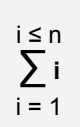
\includegraphics[width=\textwidth]{1.png}
            \end{figure}
        \subsection{Exercício 3}
            Melhor caso: $f(n) = n$ logo $O(n), \Omega(n), \Theta(n)$\\
            Pior caso: $f(n) = 2n$ logo $O(n), \Omega(n), \Theta(n)$
        \subsection{Exercício 4}
            O código realiza $(n - 3)$ operações.
        \subsection{Exercício 5}
            O código efetua $\log_2(n) + 1$ operações.
        \subsection{Exercício 8}
            Sim, porque temos que testar todos os elementos para garantir nossa resposta.
        \subsection{Exercício 9}
            Sim, porque temos que testar todos os elementos para garantir nossa resposta.
        \subsection{Exercício 10}
            O aluno deve escolher a primeira opção, pois a pesquisa sequencial tem custo $\Theta(n)$.
            A segunda opção tem custo $\Theta(n*\log_2(n))$ para ordenar, mais $\Theta(n)$ para a pesquisa binária.
        \subsection{Exercício 12}
            \textbf{Função de complexidade}

            MOV     CMP\\

            PIOR $f(n) = 2 + (n – 2) | f(n) = 1 + 2(n – 2)$
            \\MELHOR $f(n) = 2 + (n – 2) x 0 | f(n) = 1 + (n – 2)$

            \textbf{Complexidade}

            MOV CMP\\
            PIOR $O(n), \Omega(n) e \Theta(n) O(n), \Omega(n) e \Theta(n)$
            \\MELHOR $O(1), \Omega(1) e \Theta(1) O(n), \Omega(n) e \Theta(n)$


\end{document}